\section{VRTI DESIGN}

\chadded[id=zheliku]{
  VRTI established closed-loop interactive systems for scenarios requiring synchronized tactile authenticity, operational safety, and visual extensibility. It can be applied to the following three types of interaction scenarios.
}

\begin{enumerate}
  \item \texttt{High-risk skill training domains} (e.g., industrial equipment maintenance, medical surgical procedures), where RIOs preserve proprioceptive motor chains (e.g., torque transmission, tissue puncture resistance) while VIOs overlay hazardous scenario visualization and operational guidance to mitigate hands-on risks.
  \item \texttt{Complex system cognition enhancement} (e.g., science experiment pedagogy, mechanical principle demonstration), leveraging RIOs to enable physically constrained interactions (e.g., spring oscillator dynamics, chemical reaction progression) while VIOs generate multidimensional dynamic data representations (e.g., force vector decomposition, molecular structure evolution) to establish multimodal cognitive closure.
  \item \texttt{Cross-space collaborative environments} (e.g., remote equipment servicing, distributed prototype design), utilizing RIOs to synchronize local operational parameters (e.g., tool torque, interface depression depth) while VIOs construct shared digital twins to enable collaborative decision-making through bidirectional haptic-visual feedback.
\end{enumerate}


\subsection{Experiment Scenario}
\chadded[id=zheliku]{
  In collaboration with Professor XXX % 提交版需匿名
  % Xiang Hua 
  and his team from the Physics Department of XXX
  % Beijing Normal 
  University, the experimental content was determined to be the verification of the law of conservation of momentum. We selected the experiment for the following reasons:
}
\begin{enumerate}
    \item It requires simultaneous perception of force (spring), time (trajectory), and system state (mass ratios).
    \item The phenomenon involves discontinuous state changes (collisions) challenging to simulate with static props.
    \item It demonstrates core physics principles transferable to other domains.
\end{enumerate}

The experimental setup consists of two blocks, A and B, connected by a spring. Students impart an initial velocity to block B by pulling it backward, causing the system to undergo periodic motion under the spring's influence. During the experiment, students observe visualized data on a panel to study the system's motion process, thereby verifying the law of conservation of momentum. The specific experiment scenario is illustrated in Figure \ref{fig:experiment-scenario}.

\begin{figure}
  \centering
  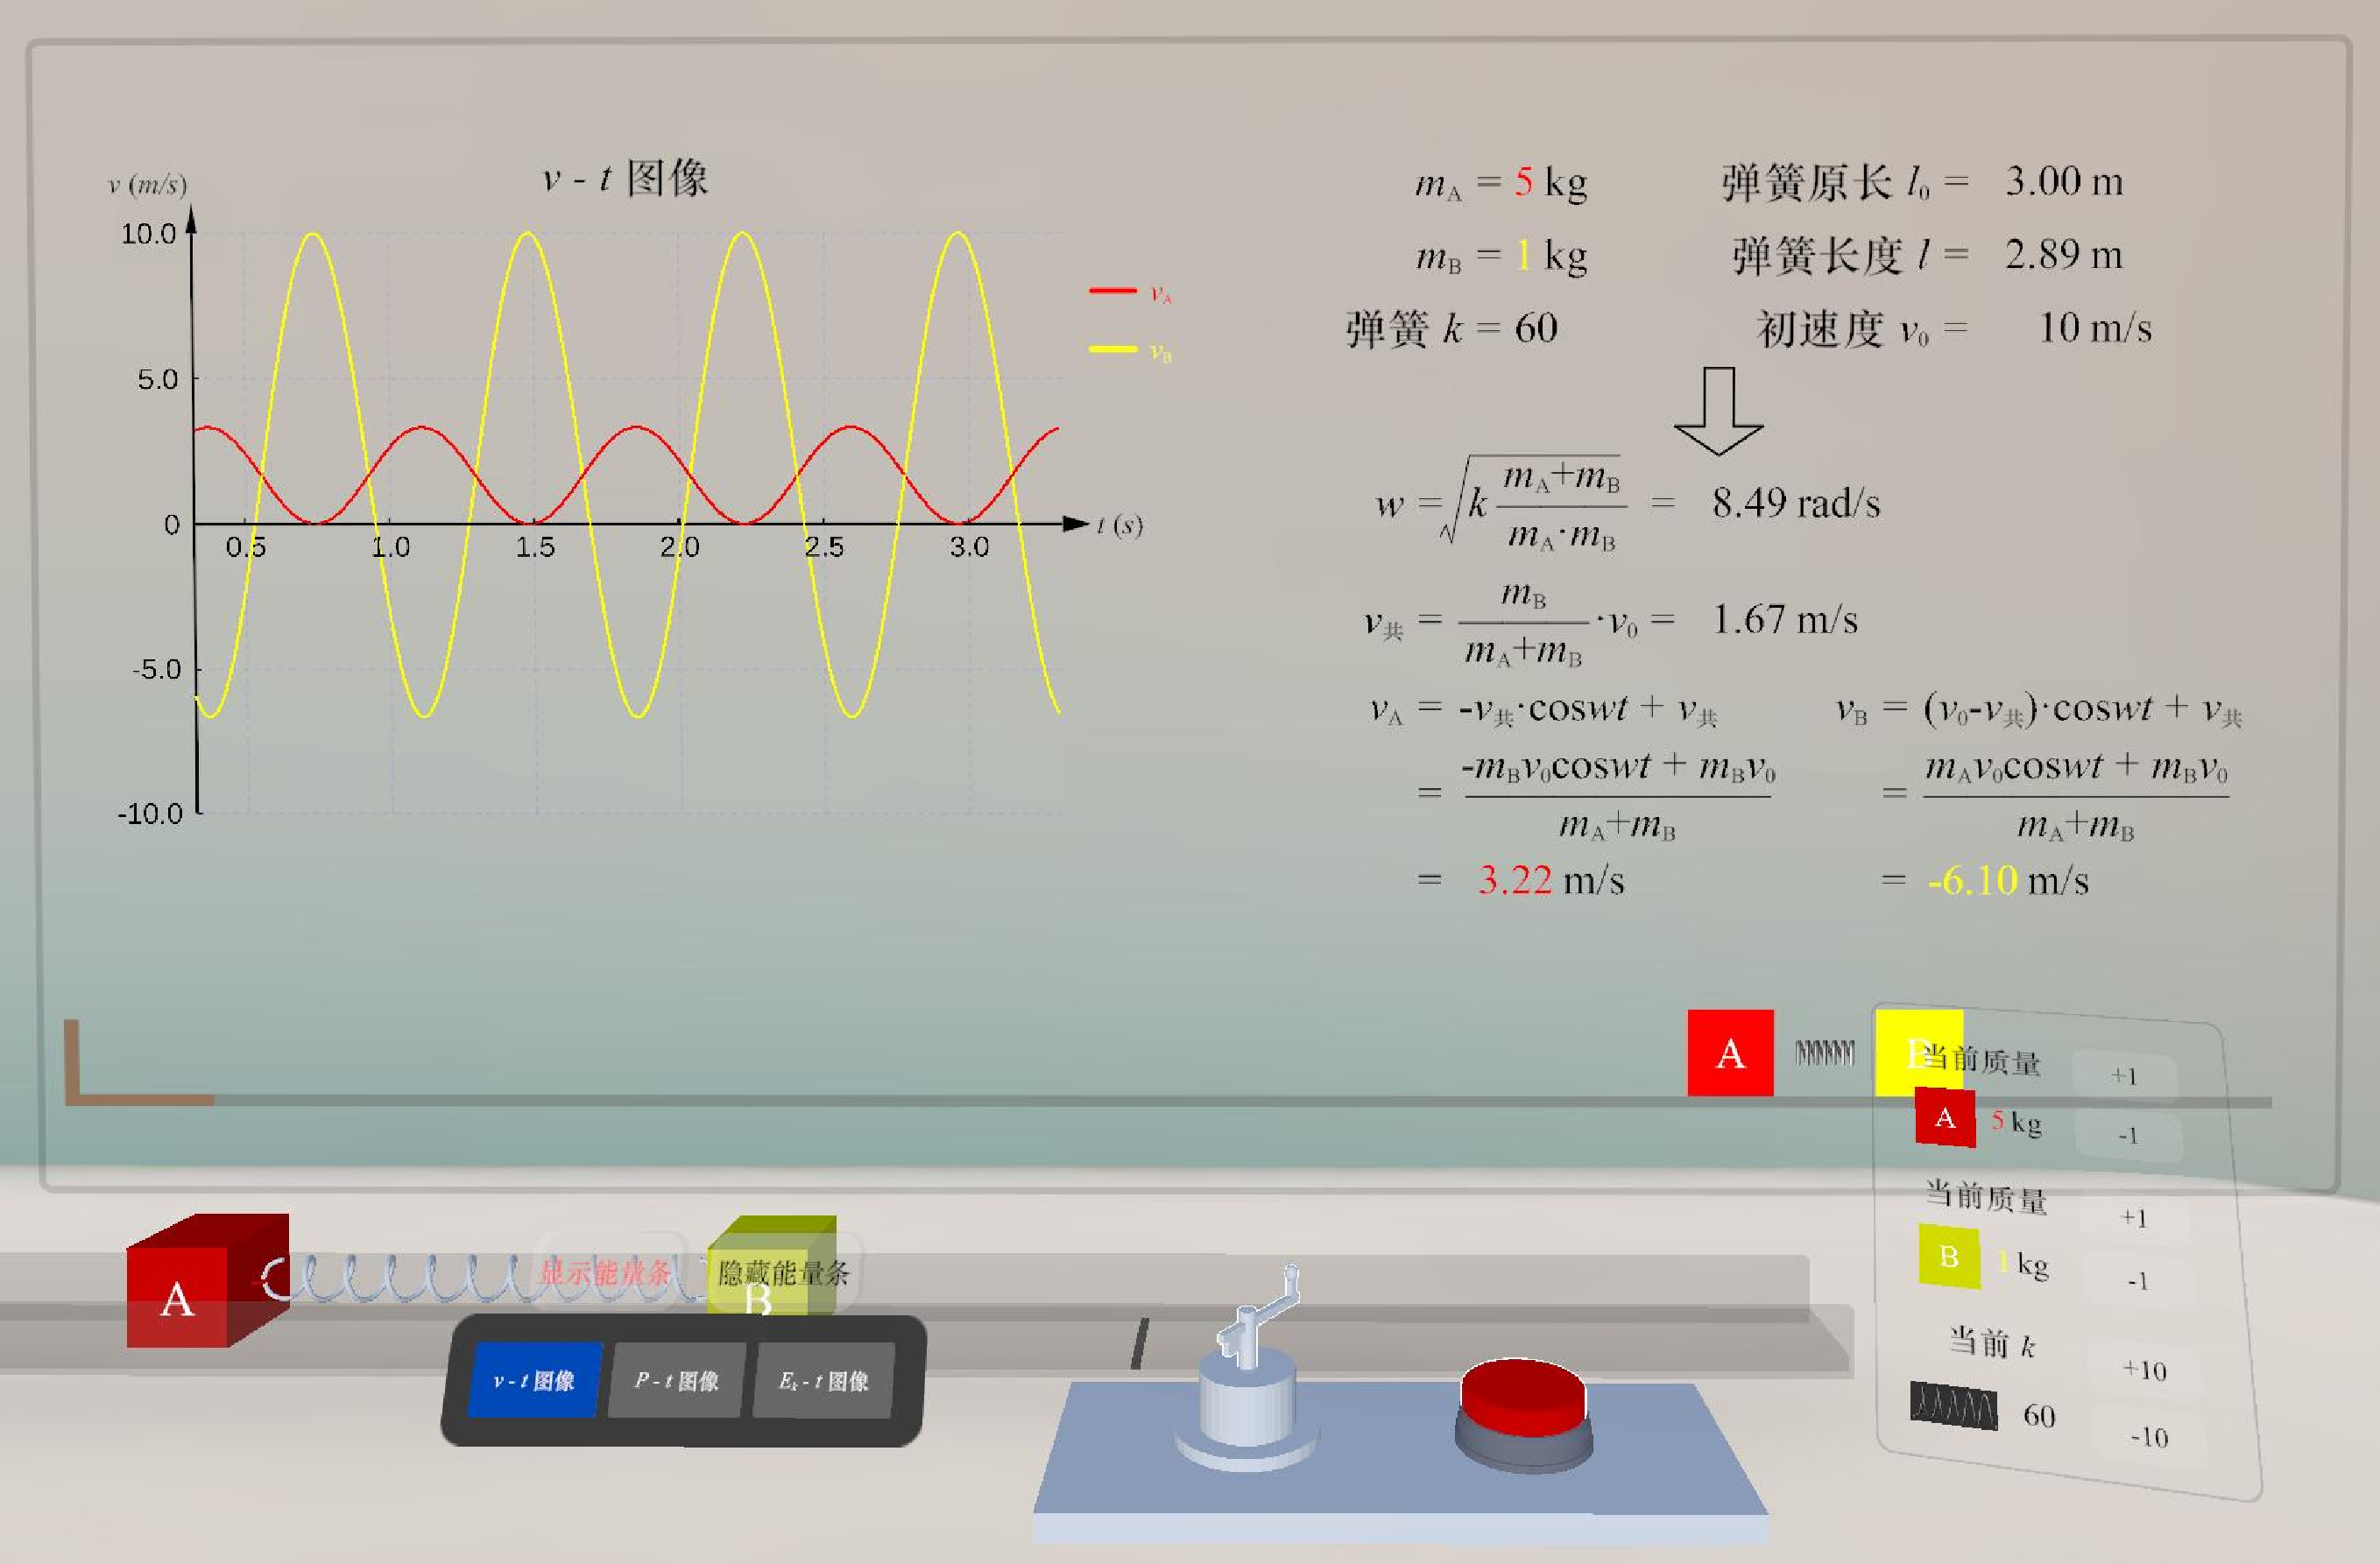
\includegraphics[width=\linewidth]{image/experiment-scenario.pdf}
  \caption{Momentum conservation experiment scenario.}
  \label{fig:experiment-scenario}
\end{figure}

Upon entering the experiment scenario, students first use their index finger to click a button on the parameter setting panel on the right to configure experimental parameters, including the masses of the two blocks and the spring constant. Next, they pull the block B to the right and release it when the force is appropriate, "launching" block B and observing the system's motion. Then, they rotate the knob to adjust the timeline of the motion process (clockwise for forward, counterclockwise for backward), exploring the characteristics of the visualized panel's graphs and the relationships between physical quantities. Finally, when the system reaches its final position, students press the button to reset the system and reconfigure the experimental parameters to continue their exploration.

On the left side of the visualization panel, three graphs: (1) $v$-$t$, (2) $P$-$t$, and (3) $E_k$-$t$ are provided to intuitively display the changes in corresponding physical quantities. The right side presents the calculation formulas for the corresponding physical quantities, showing their computational processes. Graph switching is implemented as button interactions to facilitate teaching needs during the experiment.

\subsection{Virtual-Real Twins}
Based on the experimental design for verifying the law of conservation of momentum, the implementation of VR twins includes a puller, a button, and a knob. Figure \ref{fig:structural-diagram} illustrates the structural design of each. The RIO and VIO for all three VR twins are derived from the same 3D model. The RIO is obtained through 3D printing, while the VIO is created by importing the model into Unity. Since the user's visual feedback is directly provided by the VIO, the VIO is rendered with color in the virtual environment, while the RIO remains uncolored.

\begin{figure*}[t]
  \centering
  \includegraphics[width=1\textwidth]{image/Structural-Diagram.pdf} % 使用\textwidth而非\linewidth
  \caption{Structural diagram of three VR twins.}
  \label{fig:structural-diagram}
\end{figure*}

\begin{figure*}[t]
  \centering
  \includegraphics[width=1\textwidth]{image/Interaction-Flow.pdf}
  \caption{Interaction flow of three VR twins.}
  \label{fig:interaction-flow}
\end{figure*}

\subsubsection{Puller}
The puller simulates pulling interactions and consists of a spring and a movable block. The left end of the spring is fixed, while the right end is connected to the block. Users pull the block to experience the spring's tension. A rail structure ensures the block moves along a straight path, preventing deviations during operation.

\subsubsection{Button}
The button is a common physical interaction device, allowing users to interact with the virtual environment by pressing it. It consists of a hollow cylindrical base and a slide switch, connected by a spring. When the button is pressed, the base remains stationary while the switch moves downward, compressing the spring. When released, the switch returns to its original position due to the spring's elasticity.

\subsubsection{Knob}
The knob simulates rotational interactions and comprises a base and a rotatable handle. Users rotate the handle to operate the knob. The rotational axis providing realistic rotational feedback to simulate resistance and restoring force at different angles.

\subsection{Interaction Design}
Among the three VR twins, the puller simulates pulling interactions, such as elastic rods or springs, providing tension proportional to the pulling distance. The button simulates touch and press interactions, such as keyboard keys or button triggers, providing elastic force proportional to the pressing distance. The knob simulates rotational interactions, such as dials or steering wheels, without providing significant feedback force. Figure \ref{fig:interaction-flow} illustrates the interaction flow of the three VR twins.

Due to the relatively large size of the block, the puller is designed for grasping interactions. User grasps the block, pulls the spring backward to a certain distance to trigger the puller, and then releases the block to allow the spring to rebound, completing the interaction. The button is designed for pressing interactions. User places their hand above the switch, presses it to a certain distance to activate the button, and then lifts their hand to complete the interaction. Due to the relatively small size of the handle, the knob is designed for pinching interactions. User pinches the head of the handle with their fingers, rotates it around the central axis to adjust its angle, and releases their fingers to complete the interaction. During the interaction, the button only records whether it is pressed, while the puller records both whether it is pulled and the magnitude of the force applied.